\chapter{Graphics}
\label{graphics}

\section{Java 2D Graphics}
\index{class!Graphics}
\index{Graphics}
\index{class!Frame}
\index{Frame}

This appendix provides examples and exercises that demonstrate Java
graphics.  There are several ways to create graphics in Java; the
simplest is to use {\tt java.awt.Graphics}.
Here is a complete example:

\begin{lstlisting}
import java.awt.Canvas;
import java.awt.Graphics;
import javax.swing.JFrame;

public class MyCanvas extends Canvas {

    public static void main(String[] args) {
        // make the frame
        JFrame frame = new JFrame();
        frame.setDefaultCloseOperation(JFrame.EXIT_ON_CLOSE);

        // add the canvas
        Canvas canvas = new MyCanvas();
        canvas.setSize(400, 400);
        frame.getContentPane().add(canvas);

        // show the frame
        frame.pack();
        frame.setVisible(true);
    }

    public void paint(Graphics g) {
        // draw a circle
        g.fillOval(100, 100, 200, 200);
    }
}
\end{lstlisting}
%
You can download this code from
\url{http://thinkapjava.com/code/MyCanvas.java}.

The first lines import the classes we need from {\tt java.awt}
and {\tt javax.swing}.

{\tt MyCanvas} extends {\tt Canvas}, which means that a
{\tt MyCanvas} object is a kind of {\tt Canvas} that provides
methods for drawing graphical objects.

In {\tt main} we

\begin{enumerate}

\item Create a {\tt JFrame}, which is a window that can contain the
  canvas, buttons, menus, and other window components;

\item Create {\tt MyCanvas}, set its width and height, and add it
  to the frame; and

\item Display the frame on the screen.

\end{enumerate}

{\tt paint} is a special method that gets invoked
when {\tt MyCanvas} needs to be drawn.
If you run this code, you should see a black circle on a gray
background.


\section{{\tt Graphics} methods}
\index{method!Graphics}
\index{setColor}
\index{drawOval}

To draw on the Canvas, you invoke methods on the
Graphics object.  The previous example uses {\tt fillOval}.
Other methods include {\tt drawLine}, {\tt drawRect} and more.
You can read the documentation of these methods at
\url{http://download.oracle.com/javase/6/docs/api/java/awt/Graphics.html}.

Here is the prototype for {\tt fillOval}:

\begin{lstlisting}
public void fillOval(int x, int y, int width, int height)
\end{lstlisting}

The parameters specify
a {\bf bounding box}, which is the rectangle
in which the oval is drawn (as shown in the figure).  The
bounding box itself is not drawn.

\index{bounding box}


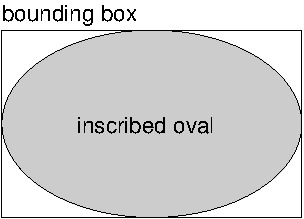
\includegraphics{figs/circle.pdf}

{\tt x} and {\tt y} specify the
the location of the upper-left corner
of the bounding box in the Graphics
{\bf coordinate system}.


\section{Coordinates}
\index{coordinate}
\index{Cartesian coordinate}
\index{graphics coordinate}

You are probably familiar with Cartesian coordinates in two
dimensions, where each location is identified by an x-coordinate
(distance along the x-axis) and a y-coordinate.  By convention,
Cartesian coordinates increase to the right and up, as shown in the
figure.


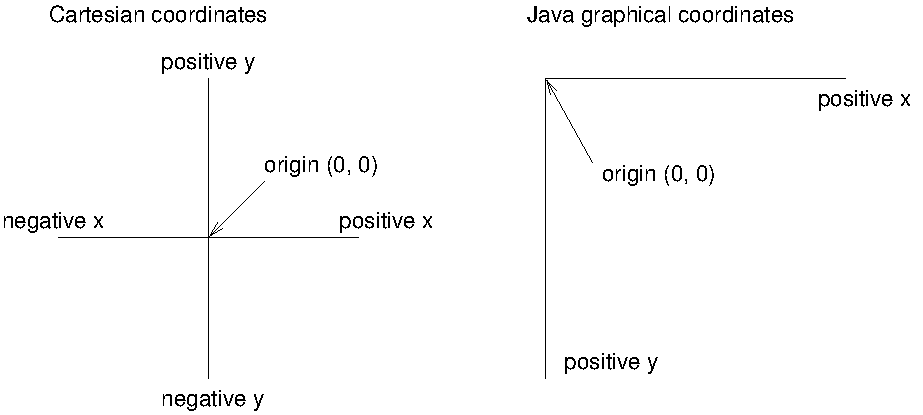
\includegraphics[width=5in]{figs/coordinates.pdf}


By convention, computer graphics systems to use a
coordinate system where the origin is in the
upper-left corner, and the direction of the
positive y-axis is {\em down}.  Java follows this convention.

\index{pixel}

Coordinates are measured in {\bf pixels}; each pixel corresponds to
a dot on the screen.  A typical screen is about
1000 pixels wide.  Coordinates are always integers.  If you want to
use a floating-point value as a coordinate, you have to round it off
(see Section~\ref{rounding}).


\section{Color}

To choose the color of a shape, invoke {\tt setColor} on the Graphics
object:

\begin{lstlisting}
    g.setColor(Color.red);
\end{lstlisting}
%
{\tt setColor} changes the current color; everything that gets drawn
is the current color.

{\tt Color.red} is a value provided by the {\tt Color}
class; to use it you have to import {\tt java.awt.Color}.
Other colors include:

\begin{verbatimtab}
black     blue    cyan   darkGray   gray   lightGray
magenta   orange  pink   red        white  yellow
\end{verbatimtab}
%
You can create other colors by specifying red, green and blue (RGB)
components.
See \url{http://download.oracle.com/javase/6/docs/api/java/awt/Color.html}.

You can control the background color of the {\tt Canvas} by
invoking {\tt Canvas.setBackground}.


\section{Mickey Mouse}
\index{Mickey Mouse}

Let's say we want to draw a picture of Mickey Mouse.  We can use the
oval we just drew as the face, and then add ears.  To make the code
more readable, let's use {\tt Rectangles} to represent bounding boxes.

Here's a method that takes a Rectangle and invokes {\tt fillOval}.

\begin{lstlisting}
    public void boxOval(Graphics g, Rectangle bb) {
        g.fillOval(bb.x, bb.y, bb.width, bb.height);
    }
\end{lstlisting}

And here's a method that draws Mickey:

\begin{lstlisting}
    public void mickey(Graphics g, Rectangle bb) {
        boxOval(g, bb);

        int dx = bb.width/2;
        int dy = bb.height/2;
        Rectangle half = new Rectangle(bb.x, bb.y, dx, dy);

        half.translate(-dx/2, -dy/2);
        boxOval(g, half);

        half.translate(dx*2, 0);
        boxOval(g, half);
    }
\end{lstlisting}

The first line draws the face.  The next three lines create
a smaller rectangle for the ears.  We translate the rectangle
up and left for the first ear, then right for the second ear.

The result looks like this:


\includegraphics[height=2in]{figs/mickey.pdf}

You can download this code from
\url{http://thinkapjava.com/code/Mickey.java}.


\section{Glossary}

\begin{description}

\item[coordinate:]  A variable or value that specifies a location
in a two-dimensional graphical window.

\item[pixel:]  The unit in which coordinates are measured.

\item[bounding box:]  A common way to specify the coordinates of
a rectangular area.

\index{coordinate}
\index{pixel}
\index{bounding box}

\end{description}


\section{Exercises}

\begin{exercise}
Draw the flag of Japan, a red circle on white background
that is wider than it is tall.
\end{exercise}


\begin{exercise}
Modify {\tt Mickey.java} to draw ears on the ears, and ears on those
ears, and more ears all the way down until the smallest ears are
only 3 pixels wide.

The result should look like Mickey Moose:

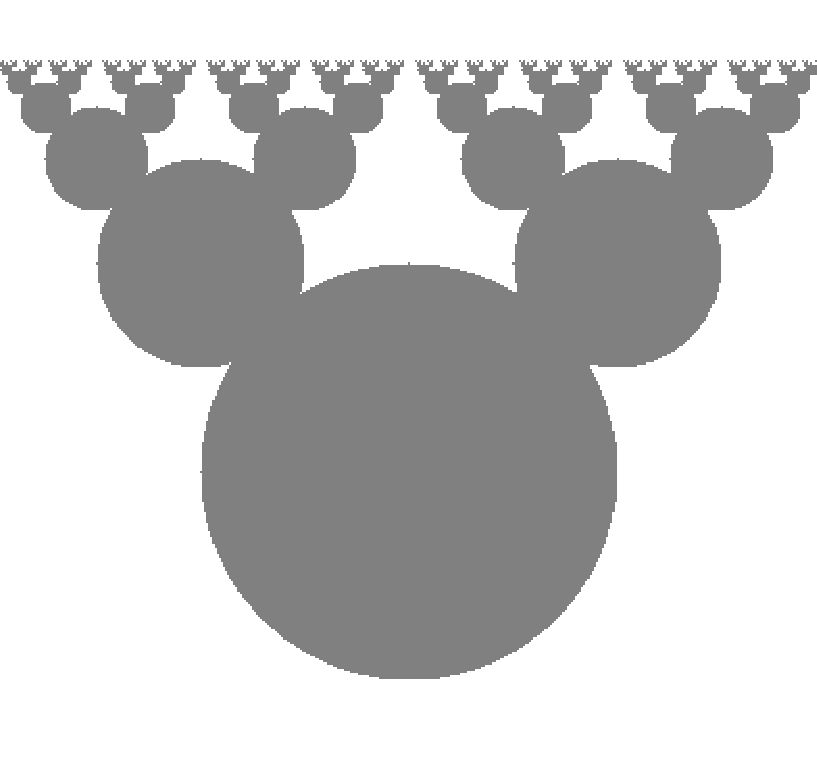
\includegraphics[height=2in]{figs/moose.pdf}

Hint: you should only have to add or modify a few lines of code.

You can download a solution from
\url{http://thinkapjava.com/code/MickeySoln.java}.

\end{exercise}


\begin{exercise}
\begin{enumerate}

\item Download
\url{http://thinkapjava.com/code/Moire.java} and import it into
your development environment.

\item Read the {\tt paint} method and draw a sketch of
what you expect it to do.  Now run it.  Did you get what you
expected?  For an explanation of what is going on, see
\url{http://en.wikipedia.org/wiki/Moire_pattern}.

\item Modify the program so that the space between the circles is
larger or smaller.  See what happens to the image.

\item Modify the program so that the circles are drawn in the center
of the screen and concentric, as in the following figure (left).
The distance between the circles should be small enough
that the Moir\'{e} interference is apparent.

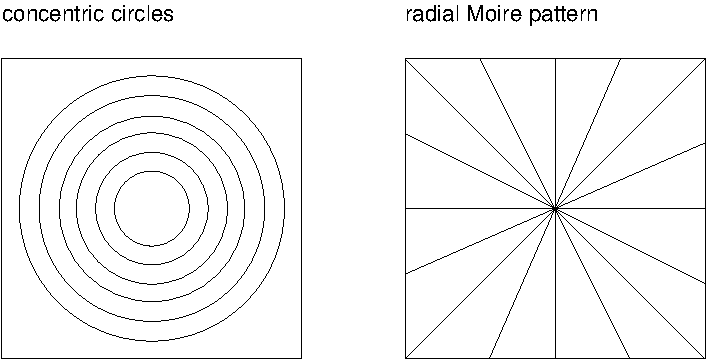
\includegraphics[height=1.5in]{figs/moire.pdf}

\item Write a method named {\tt radial} that draws a radial set
of line segments as shown in the figure (right), but they should be close
enough together to create a Moir\'{e} pattern.

\item Just about any kind of graphical pattern can generate
Moir\'{e}-like interference patterns.  Play around and see what you
can create.

\end{enumerate}
\end{exercise}


